\documentclass{article}
\usepackage[paperwidth=594mm,paperheight=841mm,top=16mm,bottom=16mm,left=19mm,right=19mm]{geometry}
\usepackage[T1]{fontenc}
\usepackage{helvet}
\usepackage{xcolor}
\usepackage{graphicx}
\usepackage{ragged2e}
\usepackage{microtype}
\usepackage{tabularx}
\usepackage{array}
\usepackage{enumitem}

\renewcommand{\familydefault}{\sfdefault}
\definecolor{ink}{HTML}{182E42}
\definecolor{blue}{HTML}{007AC3}
\definecolor{accent}{HTML}{C55A11}
\definecolor{softblue}{HTML}{EAF5FA}
\definecolor{softorange}{HTML}{FBEFE7}
\definecolor{rulegray}{HTML}{CBD5DC}
\color{ink}
\pagestyle{empty}
\setlength{\parindent}{0pt}
\setlength{\parskip}{2.5mm}
\setlength{\tabcolsep}{3mm}
\renewcommand{\arraystretch}{1.22}
\hyphenpenalty=10000
\exhyphenpenalty=10000
\setlist[itemize]{leftmargin=8mm,itemsep=1.6mm,topsep=1mm,parsep=0mm}

\newcommand{\TargetAccuracy}{50.0\%}
\newcommand{\ContextAccuracy}{55.5\%}
\newcommand{\BertAccuracy}{67.1\%}
\newcommand{\AccuracyGain}{11.6}
\newcommand{\BertMacroF}{66.7\%}
\newcommand{\ContextMacroF}{55.1\%}
\newcommand{\DifferenceLower}{-16.9}
\newcommand{\DifferenceUpper}{-6.6}
\newcommand{\ValidationCount}{638}
\newcommand{\SelectionHash}{debfd61b068f22ea1a737f238bd90ea4fb8bf44f675907e428949b559a0bb309}
\newcommand{\BertOnlyCount}{178}
\newcommand{\StaticOnlyCount}{104}
\newcommand{\BertErrorCount}{210}

% Author details supplied by the user on 2026-09-13.
\newcommand{\FirstAuthor}{Choudhary Prashant Santosh}
\newcommand{\FirstEnrollment}{1910474}
\newcommand{\SecondAuthor}{Rahul Khunt}
\newcommand{\SecondEnrollment}{1911272}


\newcommand{\bodyfont}{\fontsize{25}{31}\selectfont}
\newcommand{\smallfont}{\fontsize{22}{27}\selectfont}
\newcommand{\reffont}{\fontsize{17}{21}\selectfont}
\newcommand{\sectiontitle}[1]{%
  {\fontsize{31}{37}\selectfont\bfseries\textcolor{blue}{#1}\par}\vspace{1mm}}
\newcommand{\numbertitle}[2]{%
  {\fontsize{31}{37}\selectfont\bfseries\textcolor{accent}{#1}\hspace{2.5mm}\textcolor{blue}{#2}\par}\vspace{1mm}}
\newcommand{\questiontitle}[2]{%
  {\fontsize{18}{22}\selectfont\bfseries\textcolor{accent}{#1}\par}\vspace{-0.5mm}%
  {\fontsize{31}{37}\selectfont\bfseries\textcolor{blue}{#2}\par}\vspace{1mm}}
\newcommand{\divider}{\par\vspace{1mm}{\color{rulegray}\rule{\linewidth}{0.6pt}}\par\vspace{2mm}}
\newcommand{\ResultCallout}[2]{%
  \begin{minipage}[t]{0.31\linewidth}\centering
  {\fontsize{42}{48}\selectfont\bfseries\textcolor{blue}{#1}\par}
  {\fontsize{21}{26}\selectfont #2}
  \end{minipage}}
\newcommand{\PosterHeader}[2]{%
  \begin{center}
  \setlength{\parskip}{0.7mm}
  
\includegraphics[width=65mm]{../assets/university-trier.pdf}\par
  \vspace{2mm}
  {\fontsize{45}{51}\selectfont\bfseries #1\par}
  {\fontsize{27}{33}\selectfont\textcolor{blue}{#2}\par}
  \vspace{2mm}
  \begin{minipage}[t]{0.40\textwidth}\centering
  {\fontsize{26}{31}\selectfont\bfseries\FirstAuthor{}}\par
  {\fontsize{22}{27}\selectfont Enrollment no.\ \FirstEnrollment{}}
  \end{minipage}\hspace{5mm}%
  \begin{minipage}[t]{0.40\textwidth}\centering
  {\fontsize{26}{31}\selectfont\bfseries\SecondAuthor{}}\par
  {\fontsize{22}{27}\selectfont Enrollment no.\ \SecondEnrollment{}}
  \end{minipage}\par
  \vspace{1mm}
  {\fontsize{22}{27}\selectfont University of Trier\quad MSc Natural Language Processing\quad Trends in Natural Language Processing}
  \end{center}
  \vspace{-4mm}\divider}
\newcommand{\ReferencesBlock}{%
  {\color{rulegray}\rule{\textwidth}{0.6pt}}\par\vspace{1mm}
  {\reffont\textbf{References}\par\vspace{0.5mm}
  \begin{minipage}[t]{0.32\textwidth}\RaggedRight
  [1] Pilehvar \& Camacho-Collados (2019). \textit{WiC}. NAACL.\par
  [2] Pennington, Socher \& Manning (2014). \textit{GloVe}. EMNLP.
  \end{minipage}\hfill
  \begin{minipage}[t]{0.32\textwidth}\RaggedRight
  [3] Devlin et al. (2019). \textit{BERT}. NAACL.\par
  [4] Camacho-Collados \& Pilehvar (2018). \textit{From Word to Sense Embeddings}. JAIR.
  \end{minipage}\hfill
  \begin{minipage}[t]{0.32\textwidth}\RaggedRight
  [5] Loureiro et al. (2021). \textit{Language Models for Word Sense Disambiguation}. Computational Linguistics.\par
  [6] Haber \& Poesio (2021). \textit{Polysemy and Homonymy in Contextualised Language Models}. Findings of EMNLP.
  \end{minipage}}}


\begin{document}
\bodyfont
\PosterHeader{Static vs Contextual Embeddings for Lexical Ambiguity}{A Word-in-Context Evaluation}

\noindent
\begin{minipage}[t][560mm][s]{0.315\textwidth}\vspace{0pt}\RaggedRight
\sectiontitle{Introduction}
Many words have more than one meaning. A \textbf{bank} can be the side of a river or a place that keeps money. This is \textbf{lexical ambiguity}. Computers represent words as vectors, so we ask whether those vectors distinguish meanings in context.

\vfill
\sectiontitle{Background}
\textbf{Homonymy} means unrelated meanings, as in river bank and money bank. \textbf{Polysemy} means related meanings, as in paper as material and paper as a newspaper.

A \textbf{word embedding} is a vector learned from language. \textbf{Cosine similarity} measures how closely two vector directions align.

\textbf{Static GloVe} gives each word one vector in every sentence [2]. \textbf{Contextual BERT} creates a new vector for each occurrence using its sentence [3].

\vfill
\sectiontitle{Related work}
Earlier word sense disambiguation used dictionaries such as WordNet. Multi-sense embeddings assign several vectors to a word [4]. ELMo and BERT instead build representations from context. WiC tests whether the same word expresses the same meaning in two sentences [1]. Most competitive systems are fine-tuned. We study frozen representations.
\end{minipage}\hfill
\begin{minipage}[t][560mm][s]{0.315\textwidth}\vspace{0pt}\RaggedRight
\sectiontitle{Hypotheses}
\textbf{H1.} A static target vector cannot distinguish senses because both uses receive the same vector.

\textbf{H2.} Averaging nearby GloVe words should add a small contextual signal.

\textbf{H3.} Frozen BERT should outperform that GloVe context baseline because its target vector changes with the sentence.

\vfill
\sectiontitle{Methodology}
\textbf{Data.} SuperGLUE WiC contains \TrainCount{} training pairs, \ValidationCount{} validation pairs and \TestCount{} public test pairs without public labels.

\textbf{Systems.} We compare the GloVe target word, the average of nearby GloVe vectors within \SelectedContextWindow{}, and \texttt{bert-base-uncased} target vectors averaged over the last four layers.

\textbf{Decision.} Each sentence pair receives a cosine similarity. A training-selected threshold turns it into ``same meaning'' or ``different meaning.'' Window size, layers and thresholds use training data only. Validation is evaluated once.

\textbf{Uncertainty.} Paired confidence intervals use \BootstrapResamples{} bootstrap resamples.

\vfill
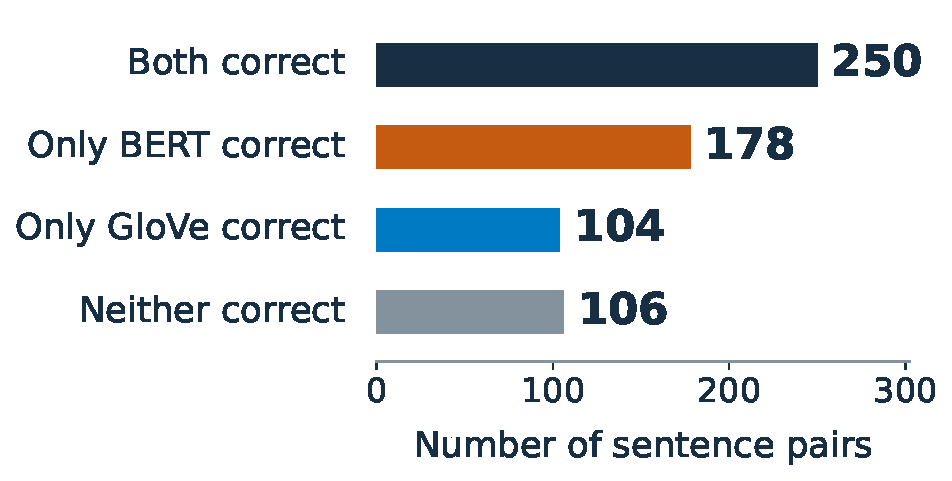
\includegraphics[width=\linewidth]{../../figures/poster_outcomes.pdf}
{\smallfont Paired outcomes show that the systems make different mistakes.}
\end{minipage}\hfill
\begin{minipage}[t][560mm][s]{0.315\textwidth}\vspace{0pt}\RaggedRight
\sectiontitle{Results}
\begin{tabularx}{\linewidth}{>{\RaggedRight\arraybackslash}X r r r}
\textbf{System} & \textbf{Acc.} & \textbf{F1} & \textbf{AUC}\\
GloVe target & \TargetAccuracy & 33.3\% & 0.500\\
GloVe context & \ContextAccuracy & \ContextMacroF & 0.580\\
BERT & \textbf{\BertAccuracy} & \textbf{\BertMacroF} & \textbf{\BertAuc}\\
\end{tabularx}

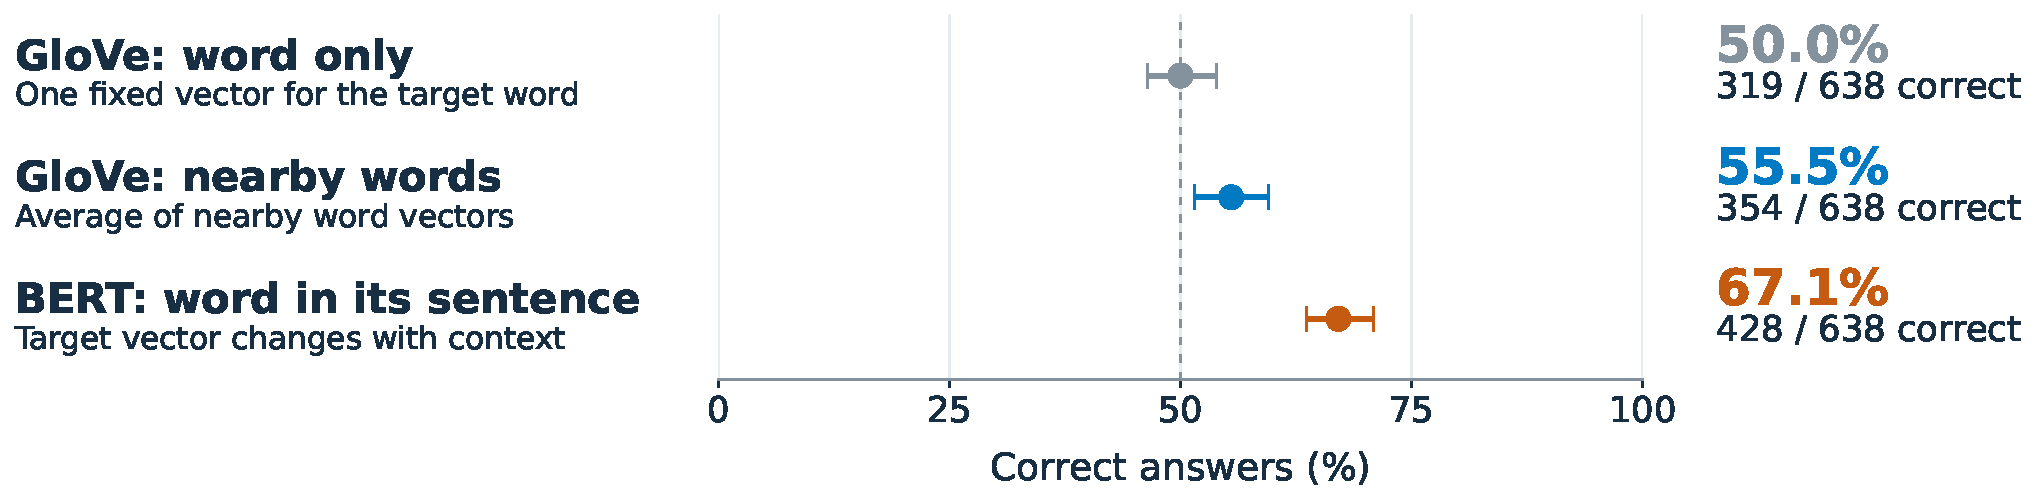
\includegraphics[width=\linewidth]{../../figures/poster_accuracy.pdf}

BERT is \textbf{\AccuracyGain{} points} more accurate than GloVe context. The paired 95\% interval is \GainLower{} to \GainUpper{} points. Layer \BestAccuracyLayer{} reaches 66.6\%, while layer \FinalLayerNumber{} reaches 63.6\%.

\vfill
\sectiontitle{Discussion}
BERT alone gets \BertOnlyCount{} pairs right. GloVe context alone gets \StaticOnlyCount{} right. BERT recovers \BertSameRecall{} of same-sense pairs but only \BertDifferentRecall{} of different-sense pairs. GloVe context shows the reverse tendency: \ContextSameRecall{} and \ContextDifferentRecall{}.

Both systems fail on difficult cases such as ``engrave a letter'' versus ``engrave a pen.''

\vfill
\sectiontitle{Conclusion}
Contextual embeddings capture sense differences better than static representations on this WiC protocol, even without fine-tuning. Yet BERT still makes \BertErrorCount{} errors. The finding is limited to one frozen model, a simple GloVe baseline and \ValidationCount{} validation pairs.
\end{minipage}

\vfill
\ReferencesBlock
\end{document}
